%%%%%%%%%%%%%%%%%%%%%%%%%%%%%%%%%%%%%%%%%%%%%%
% Head matter - can we try to be consistent on
% included packages
\documentclass{beamer}
\mode<presentation>
{\usetheme{default}
 \usecolortheme{default}
 \usefonttheme{default}
 \setbeamertemplate{navigation symbols}{}
 \setbeamertemplate{caption}[numbered]} 
\usepackage[english]{babel}
\usepackage[utf8x]{inputenc}
\usepackage{graphicx}
%%%%%%%%%%%%%%%%%%%%%%%%%%%%%%%%%%%%%%%%%%%%%%
% Formatting for title page
\title[Twitter Sentiment Analysis]{Twitter Sentiment Analysis}
\author{Christian Hotz-Behofsits, Dominik Pichler, Matthias Reisinger, Thomas Schmidleithner, Florian Taus}
\institute{Advanced Internet Computing}
\date{29th January 2015}
%%%%%%%%%%%%%%%%%%%%%%%%%%%%%%%%%%%%%%%%%%%%%%
\begin{document}
\begin{frame}
  \titlepage
\end{frame}
%\section{Introduction}
% There is actually no point to the sections 
% since we are not using table of contents mark up
\begin{frame}{Introduction}
\begin{block}{Aim}
Aggregate sentiment values of different tweets by a value specific keyword via the Twitter API.
\end{block}
\begin{itemize}
   \item Load Tweets from Twitter API
   \item Preprocessing
   \item Classification
   \item Aggregation of overall sentiment
\end{itemize}
\end{frame}

\begin{frame}{Scope of Stage 2}

\begin{itemize}
 \item Wrap sentiment analysis application into a simple Web service
 \item Provide a GUI for testing and demonstrating the service
 \item Experiment with different algorithms to improve original implementation
\end{itemize}

\end{frame}

\begin{frame}{Web service}
We implemented a RESTful Web service by the use of Spring MVC which allows to register a company 
and fetch the general feeling (sentiment) of the Twitter community about that company.
\begin{itemize}
 \item \emph{/register:} Register company 
 \item \emph{/sentiment:} Fetch sentiment of the registered company by params:
  \begin{itemize}
	\item \emph{name} - the name of the company
	\item \emph{startDate} - start date range (Format: yyyy-MM-dd)
	\item \emph{endDate} - end date range (Format: yyyy-MM-dd)
	\item \emph{classifier} - the classifier (\emph{SVM\_C\_SVC}, \emph{SVM\_NU\_SVC}, \emph{SMO}, \emph{NAIVE\_BAYES}, \emph{BAYES\_NET} or \emph{KNN})
 \end{itemize}
\end{itemize}
\end{frame}

\begin{frame}{Web interface}
A simple Web interface GUI was implemented to interact with the REST Web service
\begin{itemize}
 \item Bootstrap\footnote{http://getbootstrap.com} HTML/CSS/JS Framework
 \item AngularJS\footnote{http://angularjs.org} for REST interaction
\end{itemize}
\end{frame}

\begin{frame}{Classification Algorithms}
  \begin{itemize}
	\item Support Vector Machine C SVC
	\item Support Vector Machine Nu SVC
	\item SMO
	\item Na\"ive Bayes
	\item Bayes Net
	\item K-Nearest Neighbour
 \end{itemize}
\end{frame}

\begin{frame}{Evaluation Results}
\begin{figure}
	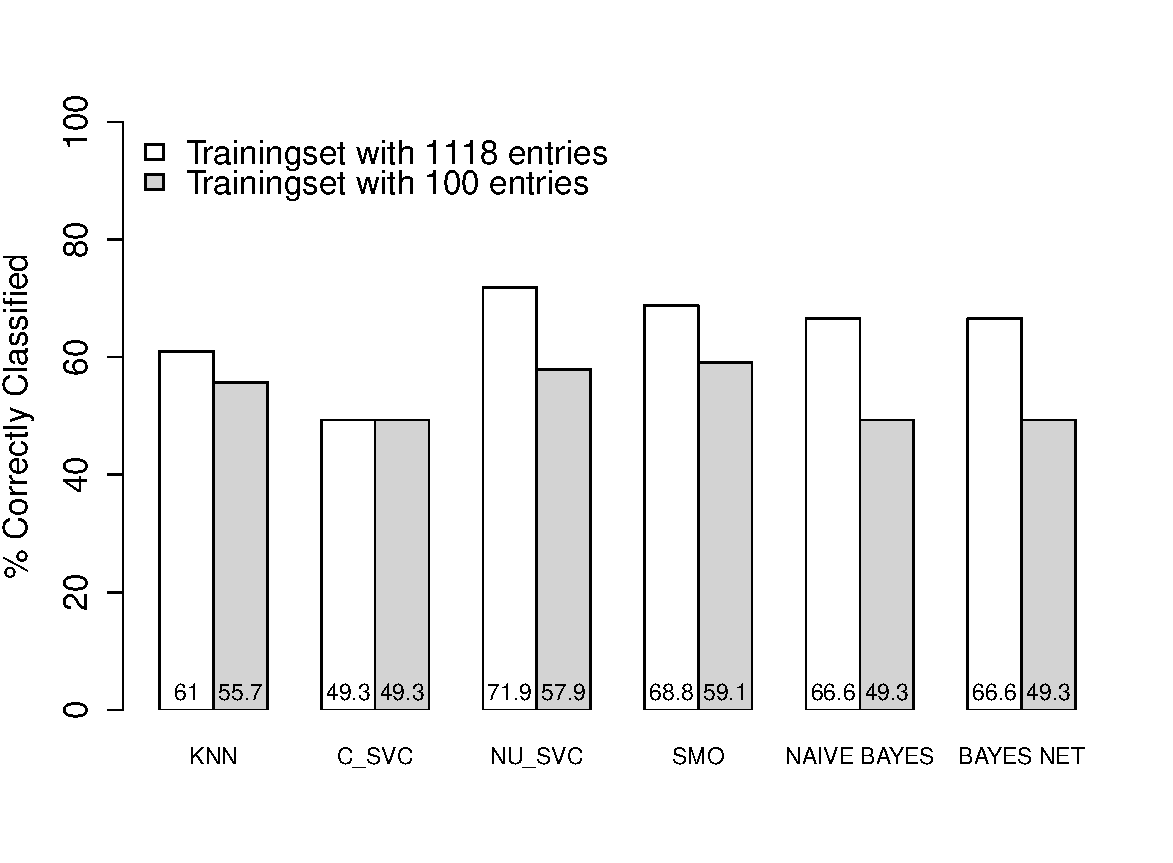
\includegraphics[width=1\textwidth]{evaluation}
\end{figure}
\end{frame}

\begin{frame}{Lessions learned/Conclusion}
\begin{itemize}
 \item Classification accuracy is strongly depended on (quality of) the training set
 \item Twitter API is very strict and restricted (search for only a few days, no time restriction possible)
 \end{itemize}
\end{frame}

\end{document}

